\section{Identifying Differential Progression in AD}\label{sec:adni}
\paragraph{Motivation.} The Alzheimer's Disease Neuroimaging Initiative (ADNI, \url{adni.loni.usc.edu})  provides a comprehensive dataset
targeted towards understanding AD. The goals of the initiative include measuring the development of the disease as a function of different imaging modalities, other biological markers, and clinical and neuropsychological assessments. 
Deep learning methods traditionally applied to this corpus require imaging data to be heavily preprocessed into summary measures, such as \textit{regions of interest}.
In other cases, based on the needs of the application (e.g., segmentation),
the approach may operate with 3D image patches instead of the entire image. 
The size of the images, especially when considered longitudinally, can be impractical for modern deep learning frameworks unless some novel
implementation tricks are utilized. 

\textbf{Data.} Our dataset consists of 522 subjects with Magnetic Resonance Imaging (MRI) scans collected over three years. For each individual, an MRI was collected annually, along with a battery of neuropsychological evaluations.

\textbf{Pre-processing.}
Full head MRIs were processed using SPM12 \cite{ashburner2014spm12}. Each image was segmented/registered using the MNI152 template. Gray matter probabilities were computed, and these gray matter density (GMD) images were used as input to our models.
The processed image size was $121 \times 145 \times 121$ (voxel size $1.5mm^3$), with \textbf{3 images per subject}.

\textbf{Model.} At this scale, we use convolutional input and deconvolutional output layers to incorporate local information with respect to reconstruction and prediction. The architecture consists of a straightforward 3-state RNN with input-hidden, hidden-hidden, and hidden-output layers replaced with TT and OTT layers. Input volumes are passed through a 3D convolutional input network, with max-pooling layers and ReLUs.
Hidden states are passed through an output convolutional network consisting of max-unpooling layers using indices
saved from the input CNN.
Strides were fixed at 1 with a kernel size of $3\times 3 \times 3$,
with successive convolutions decreasing (increasing) the number of channels by 2.
Max pooling was applied uniformly to all 3 input channels with a stride of 2. Adam optimization \cite{kingma2014adam} was used for all
ADNI experiments, with learning rate $1e^{-3}$, and decay rate $0.9$ and $0.999$ for the first and second moments. TT and OTT layers were fixed with a rank of 64. Batch sizes were fixed at 4.
%\begin{figure}
%	\centering
%	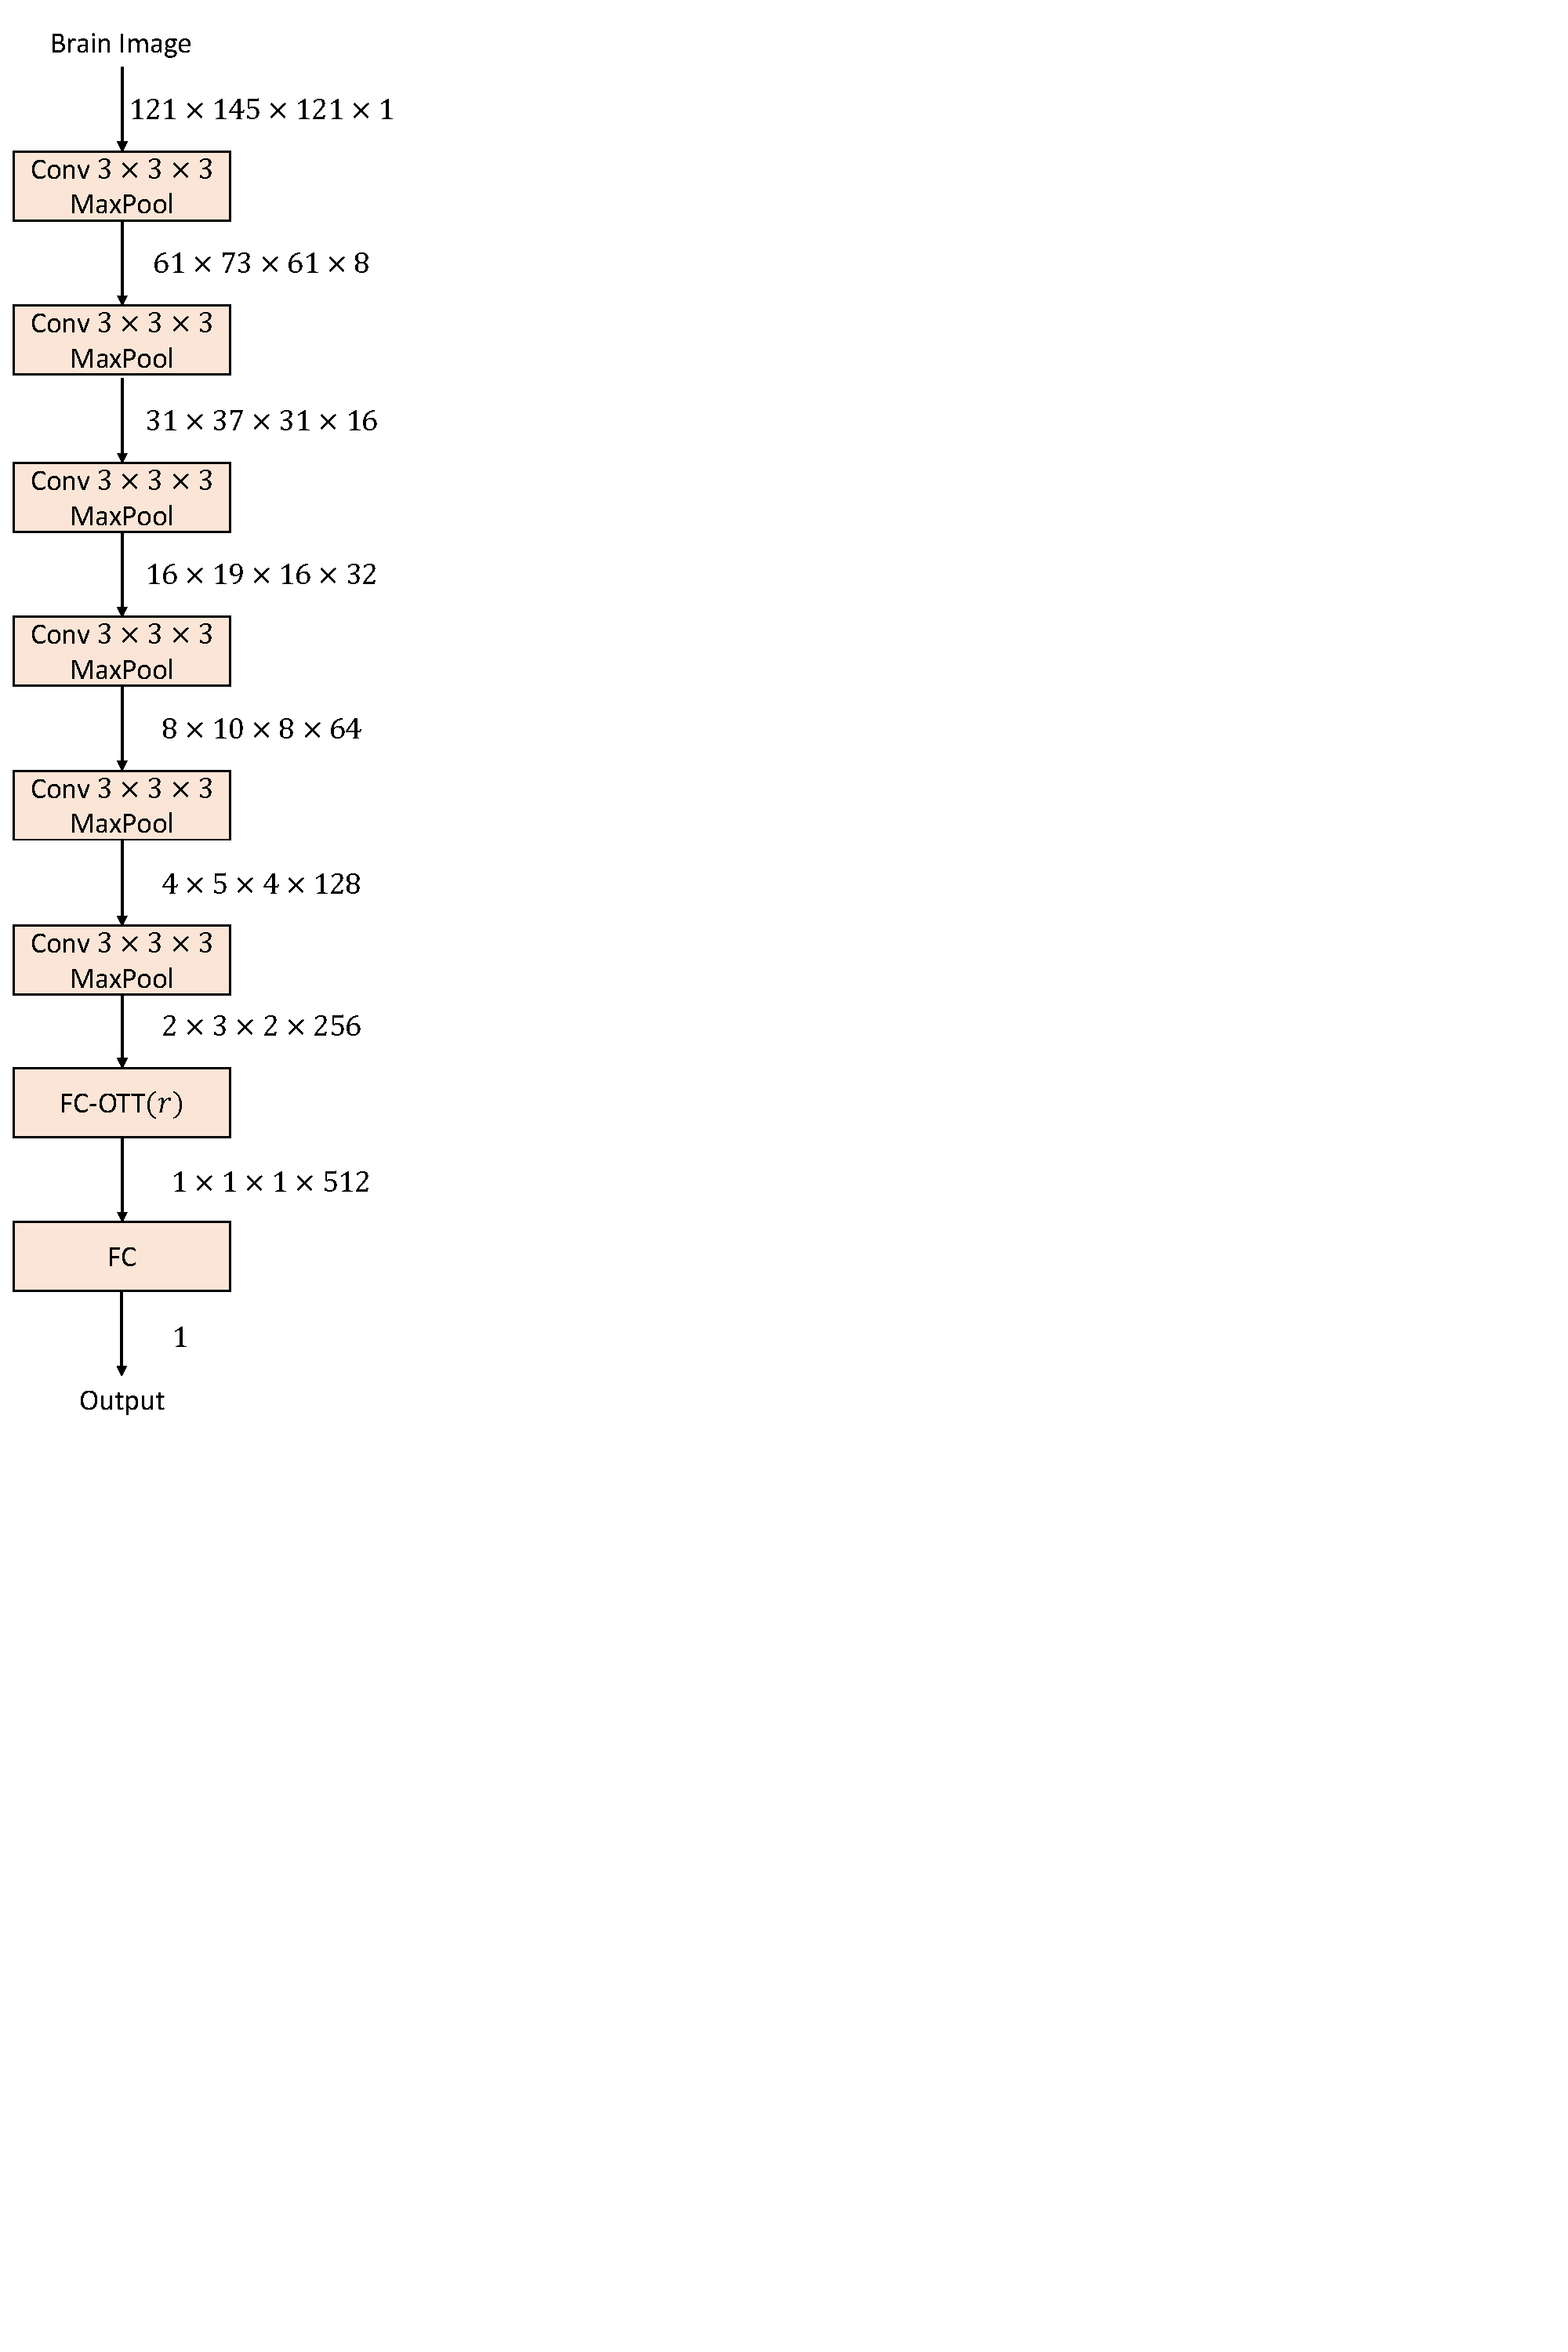
\includegraphics[angle=90,width=\textwidth,trim={0, 8in, 10in, 0}]{figs/architecture.pdf}
%\end{figure}


\subsection{Modeling gray matter progression in AD}
Our first goal is to predict the next MR image
given the previously seen ones. Importantly, standard RNN constructions cannot easily handle inputs of this size.
On a single NVIDIA Titan Xp, the images must be \textbf{downsampled} by over 20$\times$ to allow for a
batch size of 4 in a standard LSTM model with a hidden state size of 2048 (4.3 billion parameters for a full sized input map).

\textbf{Results.}
Fig \ref{fig:adpos} show the results for a held-out subject in the study using OTT-RNN on a single representative 2D slice,
with their predicted third timepoint image. While higher levels of compression (lower OTT ranks) lead to ``blocky" reconstructions,
our model is still able to identify boundaries of edges between low and high probabililty voxels.

\begin{figure}
	\centering
	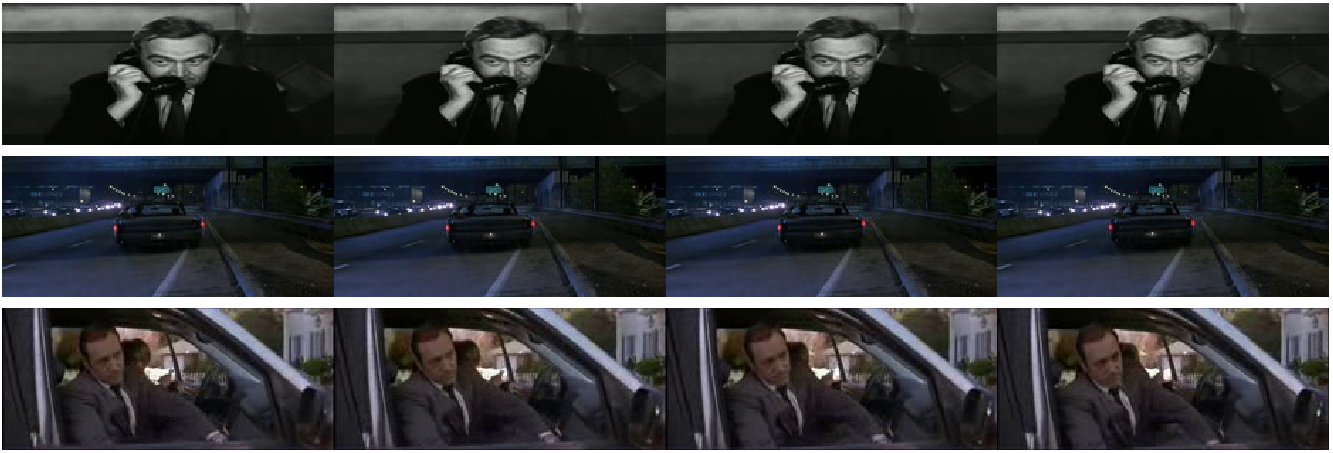
\includegraphics[width=\columnwidth]{4_ott/figs/Hollywood2_samples.png}
	\caption{\label{fig:hollywood} Sample sequences from the Hollywood2 dataset. Labels are (Top) Answer Phone, (Middle) Drive Car, and (Bottom) Get Out Car.}
\end{figure}

%
%\begin{figure}[t]
%    \centering
%    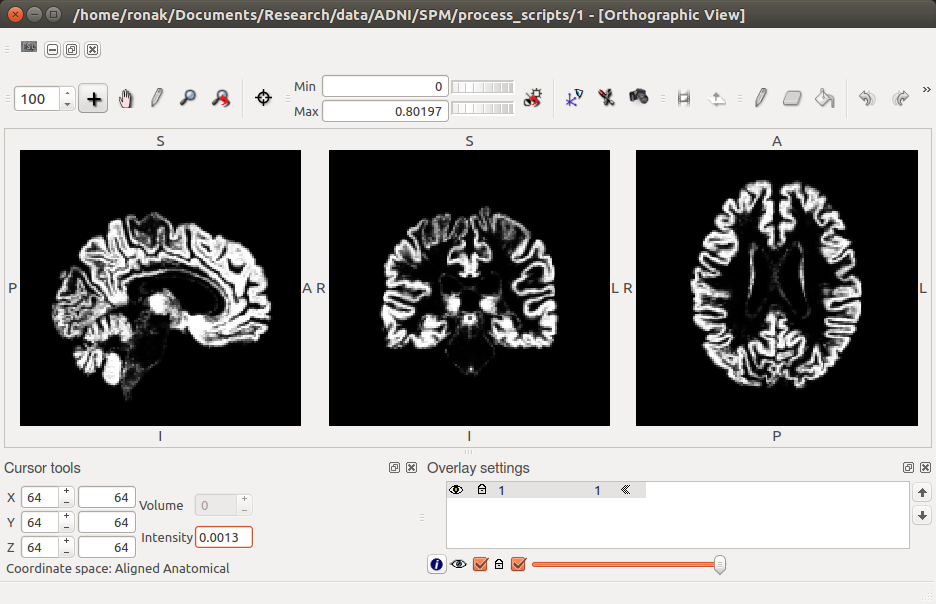
\includegraphics[width=0.98\columnwidth,trim={0 5.5cm 0 4.5cm},clip]{figs/brains/neg_1.png}
%    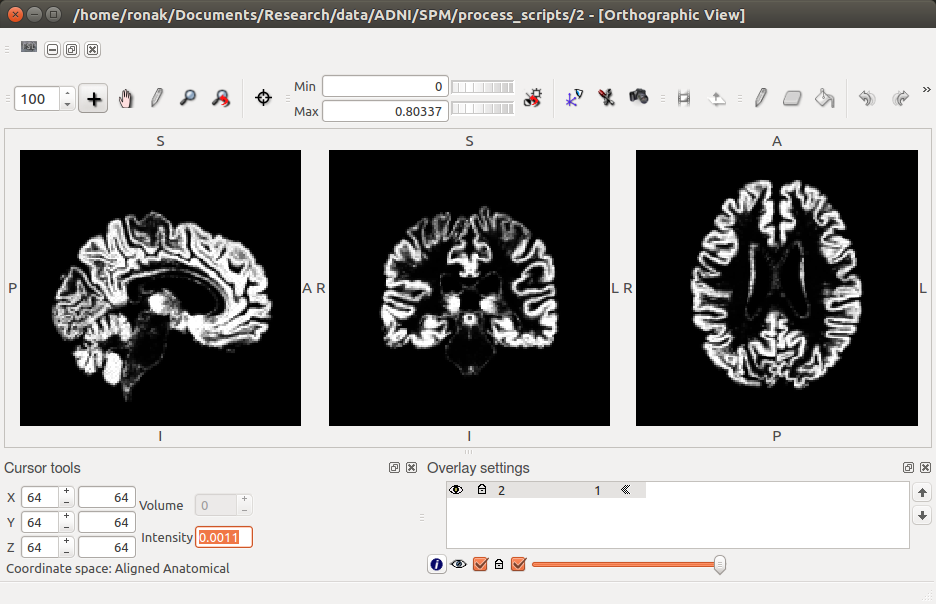
\includegraphics[width=0.98\columnwidth,trim={0 5.5cm 0 4.5cm},clip]{figs/brains/neg_2.png}
%    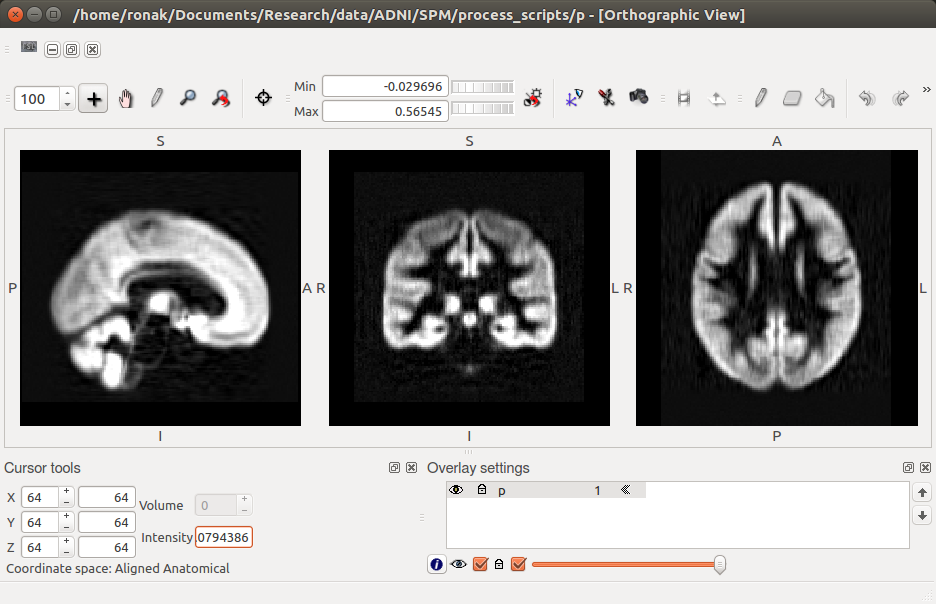
\includegraphics[width=0.98\columnwidth,trim={0 5.5cm 0 4.5cm},clip]{figs/brains/neg_p.png}
%    \caption{Ground truth progression and prediction of gray matter probabilities in an individual diagnosed as clinically normal.}
%    \label{fig:adneg}
%\end{figure}
\newcolumntype{C}{>{\centering\arraybackslash}p{0.23\textwidth}}
\begin{figure}
	\centering
	\begin{tabular}{CCCC}
		Timepoint 1 & Timepoint 2 & Timepoint 3 & \textbf{\color{blue}Predicted T3 }\\
		\multicolumn{4}{C}{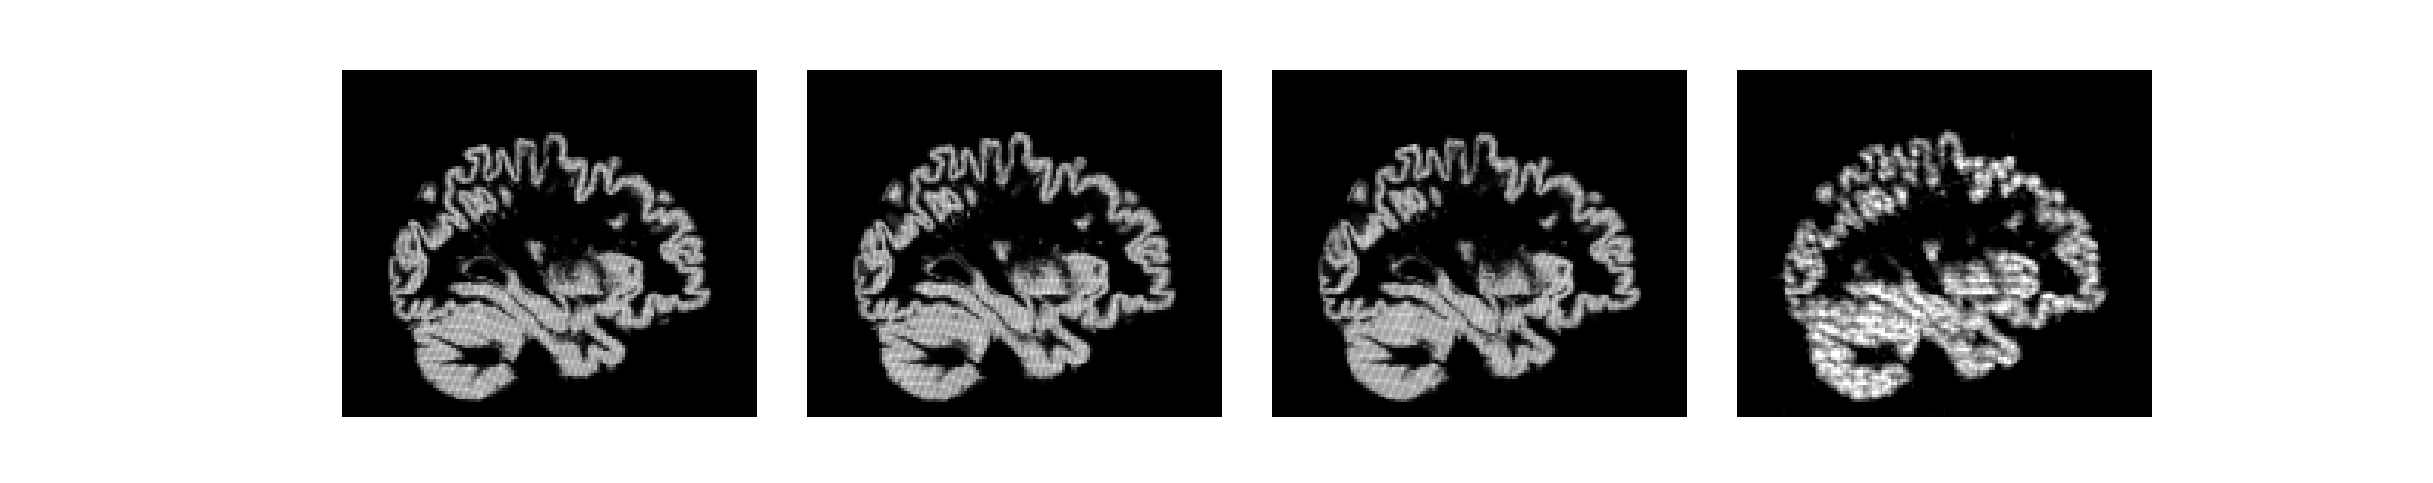
\includegraphics[width=\textwidth,trim={5cm 1cm 4cm 0.5cm},clip]{4_ott/figs/brains/ott_brain_side.eps}} \\	\multicolumn{4}{C}{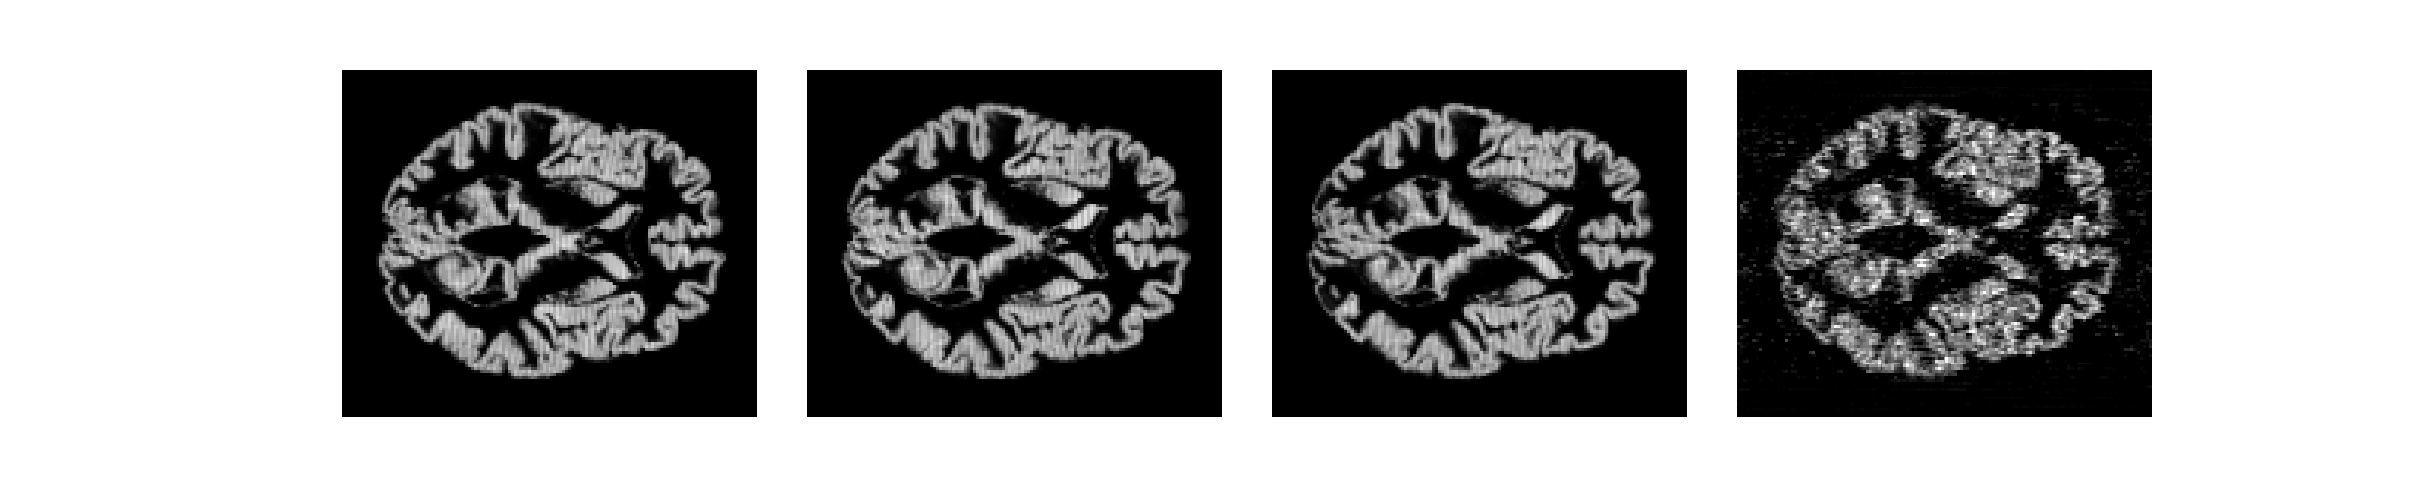
\includegraphics[width=\textwidth,trim={5cm 0.5cm 4cm 1cm},clip]{4_ott/figs/brains/ott_brain_top.eps}}
	\end{tabular}
	%    
\includegraphics[angle=90,origin=c,width=0.3\textwidth]{figs/brains/1_A.eps}
	%    
\includegraphics[angle=90,origin=c,width=0.3\textwidth]{figs/brains/2_A.eps}
	%    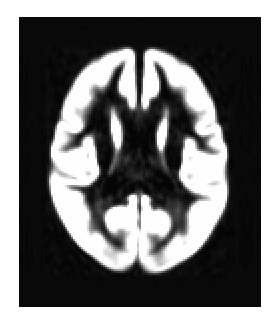
\includegraphics[angle=90,origin=c,width=0.3\textwidth]{figs/brains/p_A.eps}
	%    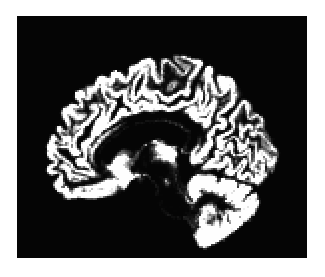
\includegraphics[width=0.3\textwidth]{figs/brains/1_S.eps}
	%    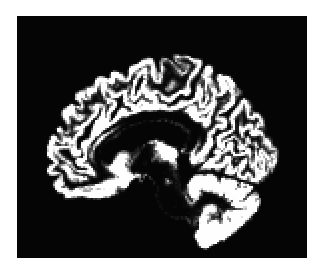
\includegraphics[width=0.3\textwidth]{figs/brains/2_S.eps}
	%    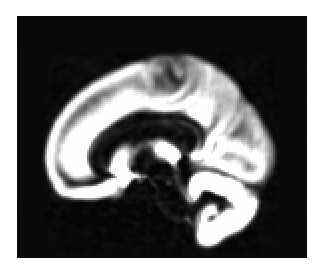
\includegraphics[width=0.3\textwidth]{figs/brains/p_S.eps}\\    
	%    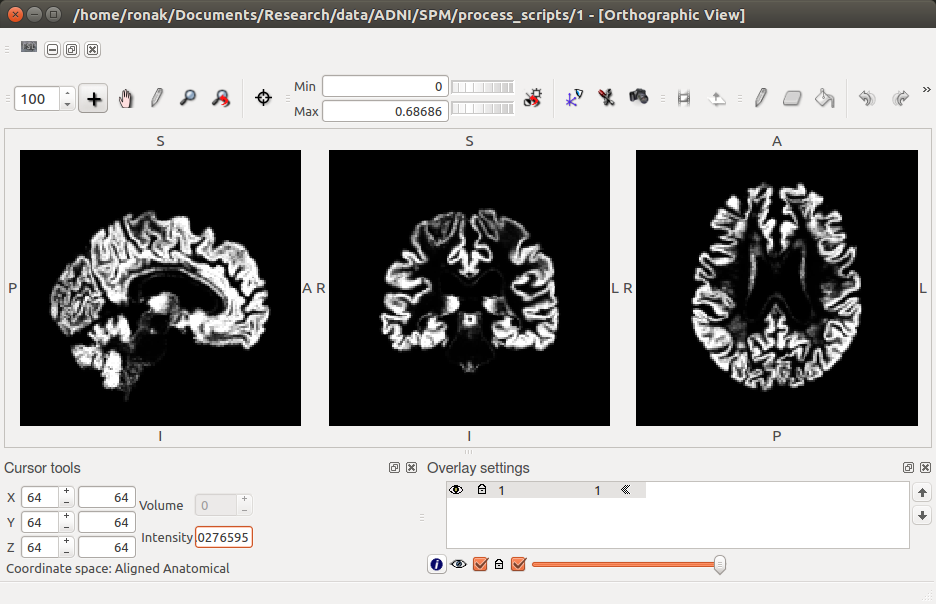
\includegraphics[width=0.75\columnwidth,trim={0 5.5cm 0 4.5cm},clip]{figs/brains/pos_1.png}
	%    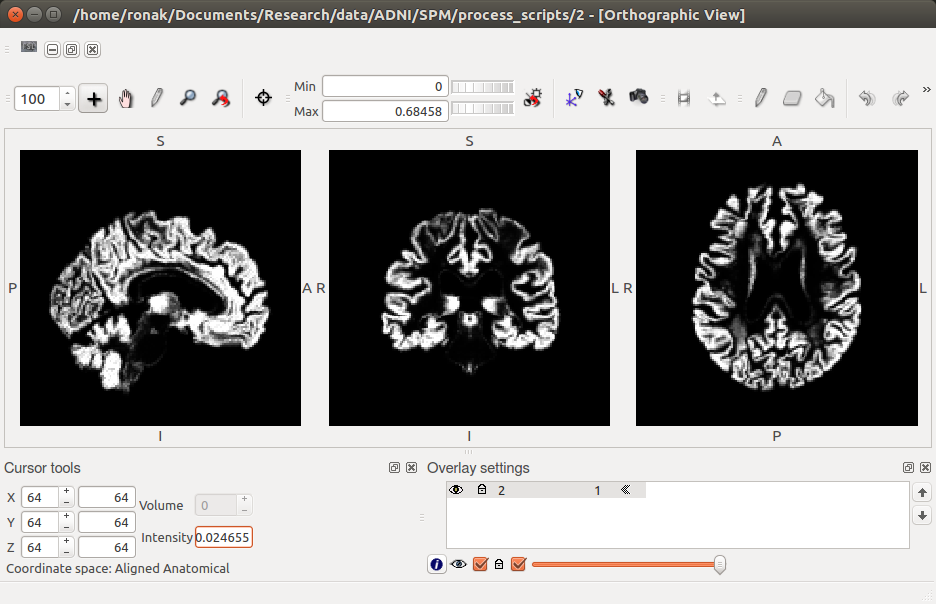
\includegraphics[width=0.75\columnwidth,trim={0 5.5cm 0 4.5cm},clip]{figs/brains/pos_2.png}
	%    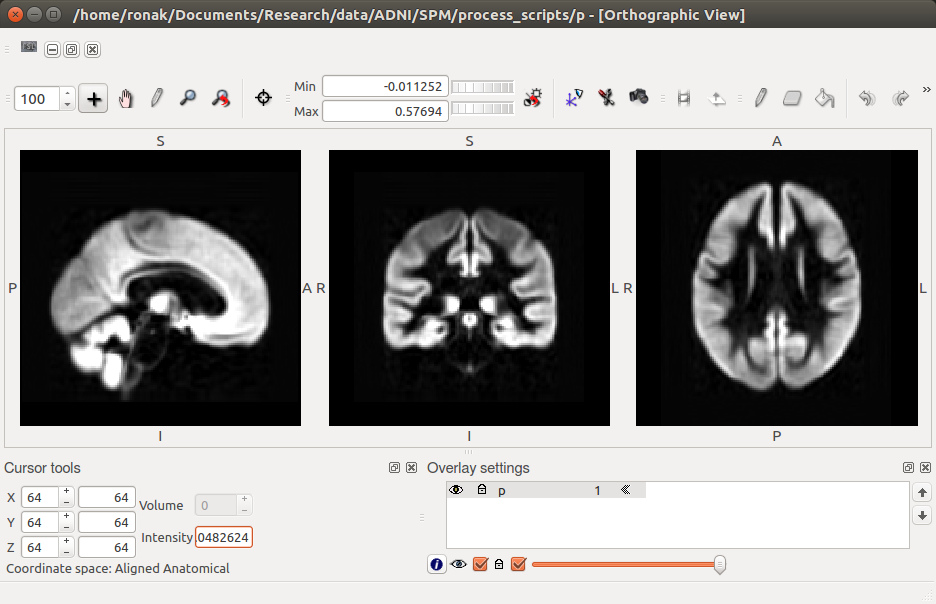
\includegraphics[width=0.75\columnwidth,trim={0 5.5cm 0 4.5cm},clip]{figs/brains/pos_p.png}
	\caption{\label{fig:adpos} Ground truth progression and prediction of gray matter probabilities in an individual from our validation set. From the left, the first three images are the ground truth images at visits 1, 2, and 3, followed by our prediction at visit 3.}
\end{figure}
\subsection{Cognition from gray matter sequence}
Based on the results from the above experiment, one may ask if, in fact, a good model of progression is being learned, or
if only the ``average'' of all participants is being predicted by the model.

\textbf{(A) Predicting Cognition from 3D image sequences.}
To answer this question, we can directly try to predict summary cognition measures which are used in practice.
%As a baseline, we first predict a subject's final disease diagnosis from their MR scans. Participants in ADNI may enter the study as cognitively healthy, but progress in their cognitive decline as time passes. We construct a binary label for each individual based on their final expert disease diagnosis, and attempt to predict it from their 3D image. Note that most of these diagnoses have occurred well after the third scan has been acquired: we are predicting \textit{future} disease condition from current and past imaging.
%Using a simple hidden layer of size 128 and an OTT/TT hidden layer, we are able to learn a model that can perfectly predict eventual AD diagnosis from MR sequences on a held out validation set.
Diagnoses themselves can often be based on partial information available
to medical experts at that time. Indeed, a small number of individuals in the ADNI cohort have been diagnosed
with AD or mild cognitive impairment and have \textit{regressed} to a cognitively healthy diagnosis at their next visit. In these situations,
categorical diagnoses can be seen as a noisy summary measure of decline.
We predict a real-valued measure collected at each timepoint.
%The Alzheimer's Disease Assessment Scale-Cognition (ADAS-Cog) has been the most widely used neuropsychological assessment in the research of Alzheimer's Disease, particularly for its design in identifying individuals who may be strong recipients of intervention \cite{skinner2012alzheimer}.
The Rey Auditory Verbal Learning Test (RAVLT) evaluates a large variety of cognitive
functions, including short and long term memory, cognitive function, and learning ability \cite{schmidt1996rey}, and
has been identified as a strong indicator for developing AD pathology. We train both TT and OTT models with dropout for 200 epochs.

\textbf{Results.} Figure \ref{fig:loss} (left) shows the results of this analysis.
Here, the advantage of the OTT construction is clear, we are able to converge significantly faster compared to the TT construction,
with half as many parameters.
\begin{figure}
	\centering
	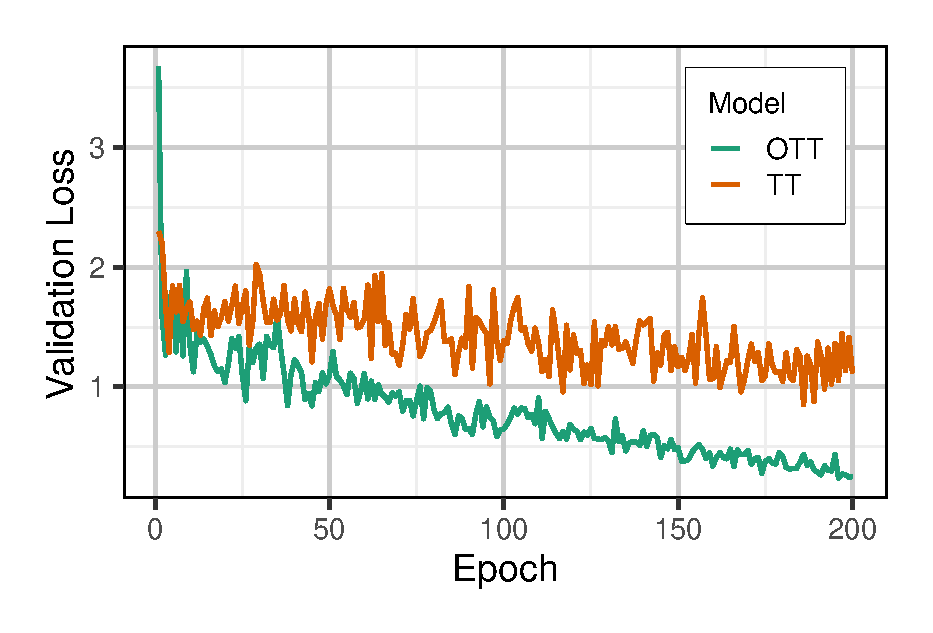
\includegraphics[width=0.49\columnwidth]{4_ott/figs/adni/adni_convergence.eps}
	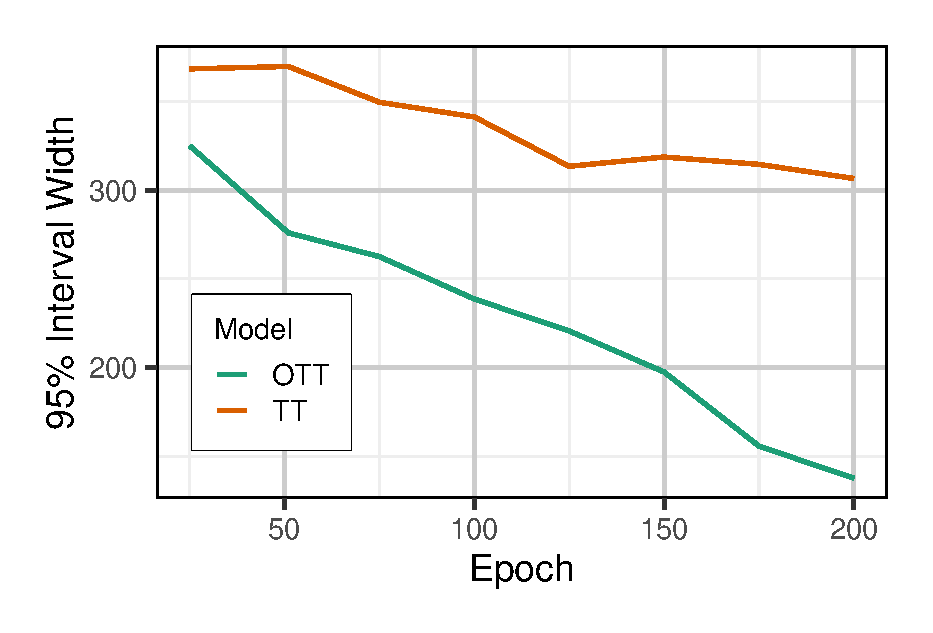
\includegraphics[width=0.49\columnwidth]{4_ott/figs/adni/adni_widths.eps}
	\vspace{-10pt}
	\caption{\label{fig:loss} \footnotesize Validation losses for reconstruction (left) and confidence interval widths (right) for uncertainty estimation of RAVLT prediction (lower is better). }
\end{figure}

\textbf{(B) Quantifying Model Uncertainty.}
Broad application of deep learning models in neuroimaging remains limited, namely due to sensitivity of black box models to mild perturbations in input data or model parameters, leading to unreliable predictions.
%Despite the impressive performance of deep learning models on many neuroimaging tasks, their widespread use in practice remains limited. As evident by a growing body of work in adversarial learning, many black box models are extremely sensitive to mild perturbations in input data or model parameters, leading to unreliable predictions.
%In classification tasks, this may be associated with the predicted probabilities indicating strong affinity towards a specific class, but with no measure of model confidence on that specific distribution. In mission critical applications from medical diagnosis to self driving cars, a confidence measure is necessary before an automated prediction model can be deployed. 
%Aleatoric uncertainty, or uncertainty that comes from noisy data or observations, is typically associated with sources external to the learning task. 
%There have been a number of recent approaches in quantifying \textit{Epistemic uncertainty}, or uncertainty resulting from the model definition or its parameters.
%However, many of these require explicit modeling of conditional distributions: infeasible for networks deployed in high-dimensional settings.
MC Dropout \cite{gal2016dropout}, approximates model (epistemic) uncertainty by using dropout \textit{at prediction time}. Simulating an ensemble of networks with different structures can yield direct estimates of uncertainty.
Obtaining good measures of this uncertainty requires sampling all parameters a significant number of times: large networks may require many samples before a reasonable uncertainty estimate.
%Monte Carlo Dropout \cite{gal2016dropout} has proven to be an effective tool in measuring model uncertainty \textit{at prediction time}. 
%Simulating an ensemble of networks with different structures can yield direct estimates of uncertainty.
%Typically, large models require a large number of samples to effectively estimate uncertainty in this manner.
%Again, we can take advantage of our reduced parameter construction.
Using tensor train constructions allows us to feasibly compute an estimate of uncertainty over all outputs, and with OTT we can further reduce this required sampling rate.

\textbf{Results.} Figure \ref{fig:loss} (right)
shows
95\% interval widths computed over 100 MC Dropout instantiations, averaged over individuals in the validation set. The advantage of our compressed orthogonal construction is clear, resulting in smaller confidence intervals compared to the standard TT decomposition. 

%results of learning the TT and OTT model for the cognition prediction task described above. For the two models, learned using an OTT hidden layer map and a TT hidden layer map, we construct 95\% confidence intervals using MC Dropout with a dropout rate of $25\%$, and sampling rate of 100.



